\documentclass{article}
\usepackage[left=3cm,right=3cm,top=3cm,bottom=3cm]{geometry}
\usepackage{amsmath,amssymb,amsthm}
\usepackage{color}
\usepackage{tikz}
\usetikzlibrary{shapes.misc,calc,arrows,matrix}

\newcommand{\MAYBE}[1]{\textcolor{red}{#1}}

\begin{document}
\title{Oral Syllabus}
\author{Li Ling Ko\\ lko@nd.edu}
\date{16 Feb 2018}
\maketitle

\section{Goal}
Prove homogeneity (Ramsey's theorem) is independent from randomness (weak
weak Konig's Lemma), under strong omnisciently computable (soc)
reducibility.

\section{Outline}
Under soc-reducibility, the only possible implications are:
\begin{center}
  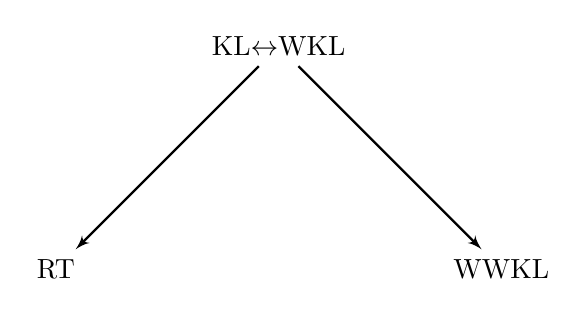
\begin{tikzpicture}[node distance=4cm,auto,thick,>=latex']
    \node (KL) {KL$\leftrightarrow$WKL};
    \node (WWKL) [below right of=KL] {WWKL};
    \node (RT) [below left of=KL] {RT};
    \draw[->] (KL) -- (RT);
    \draw[->] (KL) -- (WWKL);
  \end{tikzpicture}
\end{center}

\noindent
I will present proofs in the following order:
\begin{itemize}
  \item $\textbf{KL} \rightarrow \textbf{WKL} \rightarrow \textbf{WWKL}$
  \item $\textbf{WKL} \rightarrow \textbf{KL}, \textbf{RT}$
  \item $\textbf{WWKL} \nrightarrow \textbf{RT}$
  \item $\textbf{RT} \nrightarrow \textbf{WWKL}$
\end{itemize}

\section{References}
\begin{enumerate}
  \item Monin, Benoit, and Ludovic Patey. \textit{$\Pi_1^0$ Encodability and
    Omniscient Reductions} arXiv preprint arXiv:1603.01086 (2016).
  \item Peter Cholak's Spring 2017 lecture notes for Basic Modern Logic 2
  \item Sergei Starchenko's Fall 2016 lecture notes for Basic Modern Logic
    1
  \item Robert I. Soare. \textit{Turing Computability: Theory and
    Applications}. Springer-Verlag Berlin Heidelberg 2016.
  \item Kenneth Kunen. \textit{Set Theory}. College publications. Studies
    in logic: Mathematical Logic and Foundations, Volume 35, 2013. Sections
    1.9, 2.2, 2.4, 2.6.
\end{enumerate}

\section{Computability Theory}
\subsection{Basics}
\begin{enumerate}
  \item Primitive recursion
  \item Turing computation
  \item Kleene's $\mu$
  \item SMN theorem
  \item Halting set
  \item 1-reducibility, $m$-reducibility
  \item Rice's theorem
\end{enumerate}

\subsection{Recursively Enumerable Sets} 
\begin{enumerate}
  \item Recursion theorem
  \item Listing theorem
  \item Friedberg splitting theorem
  \item Creative sets
  \item Simple sets, hyper-simple sets
\end{enumerate}

\subsection{Relative Computability} 
\begin{enumerate}
  \item Oracle computation
  \item Finite use principle
  \item Turing degrees
  \item Jump theorem
  \item Arithmetical hierarchy
  \item Turing functionals
  \item Post's theorem
\end{enumerate}

\subsection{Degrees} 
\begin{enumerate}
  \item Low-basis theorem
  \item Incompleteness
  \item PA degrees
  \item Martin-Lof randoms
\end{enumerate}

\section{Set Theory}
\subsection{Basics} 
\begin{enumerate}
  \item Axioms
  \item Ordinals
  \item Cardinals
  \item Equivalent forms of choice
\end{enumerate}

\subsection{$V=L$} 
\begin{enumerate}
  \item Transitive closure
  \item Rank function
  \item Constructible sets
  \item Absoluteness
\end{enumerate}

\section{Model Theory}
\subsection{Structure and Theory} 
\begin{enumerate}
  \item Languages, structure, $\mathcal{L}$-homomorphisms,
    $\mathcal{L}$-embeddings, isomorphisms, substructures
  \item Terms, formulas, rules of deduction, elementary equivalence
  \item Tarski-Vaught, Lowenheim-Skolem
\end{enumerate}

\subsection{Compactness} 
\begin{enumerate}
  \item Ultrafilters, ultraproducts
  \item Los's theorem
  \item Henkin construction
\end{enumerate}

\subsection{Quantifier Elimination} 
\begin{enumerate}
  \item Definition, examples
  \item Model completeness
\end{enumerate}

\subsection{Types} 
\begin{enumerate}
  \item Realizing types
  \item Complete types
  \item Omitting types
\end{enumerate}

\subsection{Models} 
\begin{enumerate}
  \item Prime and atomic models
  \item Saturated models
  \item Vaught's theorem
  \item Homogeneous models
\end{enumerate}

\section{Combinatorics}
\subsection{Graphs}
  \begin{enumerate}
    \item Finite tres
    \item Cayley's formula
    \item Prufer codes
  \end{enumerate}

\subsection{Counting Principles}
  \begin{enumerate}
    \item Compositions
    \item Partitions
    \item Twelvefold method
    \item Generating functions
    \item Exponential formula 
    \item Inclusion-exclusion
    \item Intersecting set systems
  \end{enumerate}

\subsection{Important Numbers}
  \begin{enumerate}
    \item Binomial coefficients
    \item Catalan numbers
    \item Stirling numbers
    \item Delannoy numbers
  \end{enumerate}
\end{document}
